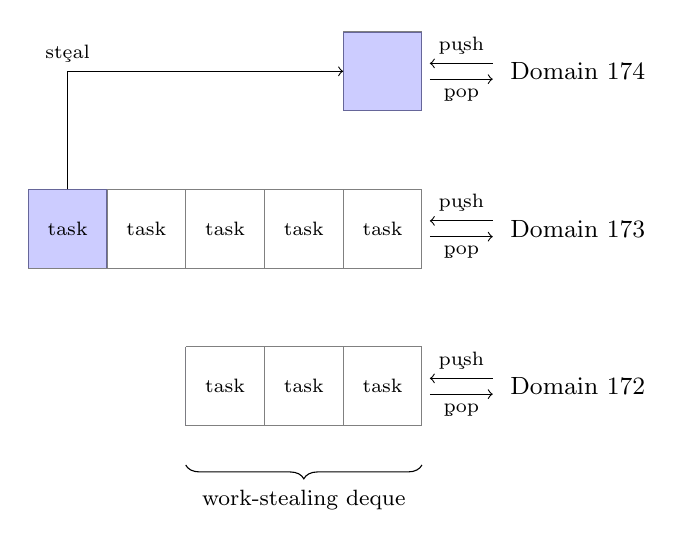
\begin{tikzpicture}
  \def\sep{1}
  \def\hsep{0.1}
  \def\vsep{0.4}
  \def\lenI{3}
  \def\lenxI{0}
  \def\lenII{4}
  \def\lenxII{1}
  \def\lenIII{0}
  \def\lenxIII{1}

  \node [right] at (1, 0.5) {\small Domain \ding{172}} ;
  \draw [step=1cm, gray] (0, 0) grid ++(-\lenI, 1) ;
  \draw [step=1cm, gray] (-\lenI, 0) grid ++(-\lenxI, 1) ;
  \fill [blue, opacity=0.2] (-\lenI, 0) rectangle ++(-\lenxI, 1) ;
  \draw [decorate, decoration={brace, amplitude=5pt}] (0, -0.5) -- ++(-\lenI, 0) node [midway, below, yshift=-2mm] {\footnotesize work-stealing deque} ;
  \draw [->] (\hsep, \vsep) -- ++(1 - 2 * \hsep, 0) node[midway, below] {\scriptsize\c{pop}} ;
  \draw [->] (1 - \hsep, 1 - \vsep) -- ++(2 * \hsep - 1, 0) node[midway, above] {\scriptsize\c{push}} ;
  \foreach \x in {1, ..., \lenI} {
  	\node at (0.5 - \x, 0.5) {\scriptsize task} ;
  }

  \node [right] at (1, \sep + 1.5) {\small Domain \ding{173}} ;
  \draw [step=1cm, gray] (0, \sep + 1) grid ++(-\lenII, 1) ;
  \draw [step=1cm, gray] (-\lenII, \sep + 1) grid ++(-\lenxII, 1) ;
  \fill [blue, opacity=0.2] (-\lenII, \sep + 1) rectangle ++(-\lenxII, 1) ;
  \draw [->] (\hsep, \sep + 1 + \vsep) -- ++(1 - 2 * \hsep, 0) node[midway, below] {\scriptsize\c{pop}} ;
  \draw [->] (1 - \hsep, \sep + 2 - \vsep) -- ++(2 * \hsep - 1, 0) node[midway, above] {\scriptsize\c{push}} ;
  \foreach \x in {1, ..., \lenII} {
  	\node at (0.5 - \x, \sep + 1.5) {\scriptsize task} ;
  }
  \node at (0.5 - \lenII - \lenxII, \sep + 1.5) {\scriptsize task} ;

  \node [right] at (1, 2 * \sep + 2.5) {\small Domain \ding{174}} ;
  \draw [step=1cm, gray] (0, 2 * \sep + 2) grid ++(-\lenIII, 1) ;
  \draw [step=1cm, gray] (-\lenIII, 2 * \sep + 2) grid ++(-\lenxIII, 1) ;
  \fill [blue, opacity=0.2] (-\lenIII, 2 * \sep + 2) rectangle ++(-\lenxIII, 1) ;
  \draw [->] (\hsep, 2 * \sep + 2 + \vsep) -- ++(1 - 2 * \hsep, 0) node[midway, below] {\scriptsize\c{pop}} ;
  \draw [->] (1 - \hsep, 2 * \sep + 3 - \vsep) -- ++(2 * \hsep - 1, 0) node[midway, above] {\scriptsize\c{push}} ;

  \draw [->, to path={|- node[above] {\scriptsize\c{steal}} (\tikztotarget)}] (0.5 - \lenII - \lenxII, \sep + 2) to (- \lenIII - \lenxIII, 2 * \sep + 2.5) ;
\end{tikzpicture}
